\documentclass[11pt]{article}
\usepackage[margin=1in]{geometry}
\usepackage[T1]{fontenc}
\usepackage{lmodern}
\usepackage{amsmath,amssymb,booktabs,graphicx,microtype}
\usepackage[colorlinks=true,linkcolor=blue,urlcolor=blue,citecolor=blue]{hyperref}
\usepackage{enumitem}
\setlist{nosep}
\newcommand{\OpCount}{28}
\newcommand{\SkipCount}{28}
\newcommand{\ScenarioCount}{108}

\title{Phase-Aware Low-Precision Inference on Commodity Hardware\newline and Auditable Architecture Exploration}
\author{Dr. Lin Wang\\\small Working paper}
\date{September 11, 2026}
\begin{document}
\maketitle
\noindent\small This draft reflects the current repository state as of September 11, 2026 and is intended for internal review before external submission.
\begin{abstract}
Hardware-aware quantization is meaningful only when execution phase, model scale,
and memory behavior are measured together. EdgeDecode is a reproducible artifact
that separates measured runtime from hypothetical architecture scenarios. On an
Apple M4 Pro, official F16, Q8\_0 and Q4\_K\_M variants of Qwen2.5-1.5B-Instruct
show a phase-dependent crossover: Q4\_K\_M improves 128-token decode by 1.95$\times$
on CPU and 2.25$\times$ on Metal, whereas F16 remains fastest for 2048-token
prefill. A 72-case sweep across 1.5B and 7B Qwen2.5 GGUFs shows that this
boundary moves with model scale, prompt length, and token-block size rather than
remaining fixed. Q8\_0 remains close to F16 in quality, while Q4\_K\_M increases
WikiText-2 perplexity by 3.94\% and reduces a 200-task HellaSwag subset by 1.5
points, with overlapping confidence intervals. These results argue against a
universal low-precision recommendation and instead motivate phase-aware software
selection for prefill and decode. The artifact also provides native reference
kernels, synthetic constrained search, and \ScenarioCount{} disclosed but
uncalibrated architecture scenarios. We report no measured power, Arm GPU/NPU
performance, or synthesized area.
\end{abstract}

\section{Introduction}
A resource-constrained inference system does not consume a nominal bitwidth in
isolation. It consumes packed weights, scales, activations, instructions, memory
transactions, and synchronization. Reducing weight storage can increase decode
work; reducing quantization group size can improve numerical fidelity while
increasing metadata. A hardware feature that accelerates one stage may have little
impact if another stage dominates. These interactions motivate a joint algorithm,
software, and architecture investigation rather than a single compression result.

The central question of this work is deliberately narrow: \emph{when do grouped
low-precision linear operators justify their representation and execution costs,
and what evidence would justify a distinct decode-optimized implementation?} A
complete answer would require pretrained models, optimized kernels,
target-specific compilation, and calibrated power and area evidence. The present
release establishes a reproducible pilot and makes explicit which parts of that
answer remain unsupported.

We distinguish three quantities throughout this study: prompt length $P$,
generation length $G$, and token-block size $B$. Prompt length denotes the number
of input tokens already present in the context window; generation length denotes
the number of tokens produced during decode; and token-block size denotes the
software batching limit used by llama.cpp during prefill or decode. These
definitions are required because the same nominal workload can exhibit different
performance under different blocking strategies, even when the underlying model and
hardware are unchanged.

As a direct end-to-end validation of the execution path, we also ran the locally
available Qwen2.5-7B Q4\_K\_M GGUF through llama.cpp on this host. The model
successfully generated the response: "EdgeDecode is an edge computing solution
that decodes and processes media content locally, reducing latency and improving
performance for real-time applications." This confirms that the real GGUF +
llama.cpp generation stack is functional, even though the repository's lightweight
agent-evaluation harness remains an explicit harness rather than a full benchmark
suite. We do not interpret this output as a quality benchmark; it is a smoke test
of the end-to-end model-serving path.

Our artifact makes three contributions. First, it specifies and implements a
packed-weight format whose CPU execution can be independently compared with an
unpacked numerical reference. Second, it evaluates complete synthetic-network
outputs while selecting configurations using measured operator costs. Third, it
separates hypothetical architecture sensitivity from real measurements, including
an explicit extra-area budget instead of a fabricated circuit-area estimate. The
pilot preserves negative findings: its quality constraint excludes mixed bitwidths,
and the low-bit kernel is not uniformly faster than its F32 counterpart.

\paragraph{Scope of evidence.}
System queries identify the host as a 12-core Apple M4 Pro with 24 GB unified memory
and a 16-core Apple GPU. Unique identifiers are excluded from the manifest. The
custom CPU backend remains a single-thread C reference without explicit intrinsics.
The llama.cpp CPU and Metal paths are optimized external baselines, but their
dominant kernels have not yet been instruction-profiled. Apple Metal is an
accelerator case study, not Arm GPU evidence. There are no Arm NPU results,
measured energy data, or synthesized area estimates. This is a technical working
draft, not an arXiv publication or a peer-reviewed claim.

\section{Background and Related Work}
Hardware-aware mixed-precision selection predates this artifact. HAQ explicitly
incorporates hardware feedback into quantization-policy search~\cite{haq}. Our
small exhaustive search is not a replacement for that research contribution: it
uses three synthetic layers, six choices per layer, and an additive measured CPU
cost. The purpose is to make the constraint and evidence chain inspectable.

AWQ couples activation-aware weight quantization with implementation choices for
on-device inference~\cite{awq}. EdgeDecode does not implement AWQ's transformations
and does not reproduce its model-level evaluation. We use a simpler symmetric
format to expose the interaction between scales, group size, packed access, and
runtime. Comparison against an established optimized method is an explicit next
step rather than an implied result.

The Roofline framework relates operational intensity to compute and data-transfer
limits~\cite{roofline}. We extend a simplified maximum-stage expression with a
decode-throughput term for illustrative sensitivity analysis. This expression
assumes ideal overlap and is not a fitted predictor of the measured CPU code.
Production-oriented libraries such as KleidiAI are relevant future baselines for
Arm-targeted kernels~\cite{kleidiai}; our scalar implementation should not be
interpreted as their attainable performance.

\section{Representation and Execution}
\subsection{A fully specified grouped format}
Let $W\in\mathbb{R}^{M\times K}$, and let a group contain $G$ consecutive weights
within a row. We pad the reduction dimension to
$K_p=G\lceil K/G\rceil$. For bitwidth $b\in\{4,8\}$ define
$q_{\max}=2^{b-1}-1$. A nonzero group uses scale
$s=\max_j|w_j|/q_{\max}$ and quantized integers
\begin{equation}
q_j=\operatorname{clip}\!\left(\operatorname{rint}(w_j/s),
-q_{\max},q_{\max}\right).
\end{equation}
Zero groups use $s=1$. Rounding follows NumPy's nearest-even rule. The unsigned
stored code is $q_j+q_{\max}$; the highest code is unused. Four-bit codes are
packed low nibble first. Scales use FP32; activations and accumulators also use
FP32. This is an artifact-specific format, not GGUF, AWQ, or a vendor ABI.

The exact weight payload, including scale metadata and padding, is
\begin{equation}
B_W=M K_p b/8+4M\lceil K/G\rceil.
\label{eq:bytes}
\end{equation}
For divisible dimensions, the scale overhead is $32/G$ bits per weight. At
$G=32$, a nominal 4-bit format therefore uses 5 bits per weight, before host object
metadata. Reporting only the nominal precision would omit a material part of the
representation cost.

\subsection{Reference execution paths}
The C operator computes $Y=X\widehat W^T$. Within each output element it decodes
integer codes, accumulates an activation dot product for each group, and applies
the group's scale. It does not expand the entire weight matrix before execution.
The F32 baseline follows the same simple row-dot structure and does not call BLAS.
The compiler is invoked with optimization enabled but without explicit
architecture intrinsics or a fast-math option.

The optional Metal kernel assigns an output element to a thread and uses persistent
shared buffers. Compilation and initial buffer construction are outside the timed
operator call. A completed GPU call would include command submission, waiting, and
output copying. Since GPU execution was unavailable, the source is delivered as an
unvalidated optional backend, and no GPU timing appears in our measured results.

\subsection{Correctness before timing}
Every measured operator is compared with NumPy multiplication using the unpacked
quantized weights. Thus a low-bit error relative to original weights is distinct
from an implementation error relative to the quantized representation. Tests cover
zero groups, non-multiple tails, storage size, invalid inputs, endpoint codes,
quantization error bounds, and composed execution. The quantized native operator is
checked with FP32 tolerances that allow different reduction orders.

\section{Quality-Constrained Configuration Selection}
For layer $\ell$, a configuration $c_\ell$ selects a bitwidth and group size from
$\{4,8\}\times\{32,64,128\}$. Given a development set $D$, we use relative output
MSE as a proxy:
\begin{equation}
Q_D(c)=\frac{\sum_{x\in D}\|f(x)-f_c(x)\|_2^2}
{\max(\sum_{x\in D}\|f(x)\|_2^2,10^{-30})}.
\end{equation}
This is not language-model accuracy. It measures agreement with an untrained
floating-point synthetic network. We evaluate the complete composition for every
candidate rather than adding independent layer errors.

Let $\widehat T_\ell(c_\ell)$ be the median measured CPU time for that layer at
$N=1$. Selection solves the finite problem
\begin{align}
\min_c\quad &\sum_\ell\widehat T_\ell(c_\ell)\\
\text{subject to}\quad &Q_D(c)\leq 0.005,\qquad
\sum_\ell B_{W,\ell}(c_\ell)\leq 0.30 B_{\mathrm{F32}}.
\end{align}
We enumerate all $6^3=216$ possibilities. This provides an exact minimum of this
\emph{finite proxy objective}, not a guarantee of minimum composed runtime.
Allocations, Python dispatch, intermediate copies and nonlinearities can invalidate
the additive timing approximation. Selected networks are consequently timed as
complete native compositions, and tested on separate inputs.

The baselines are uniform Q4/G128, uniform Q8/G64, a quality-only minimum under the
same storage constraint, and a uniformly sampled feasible configuration. The random
control is constrained by quality and maximum storage; it is not exactly
byte-matched. All baselines share generated weights and input splits. An identical
configuration may be selected by multiple rules. Its separately measured times
should be read as repeated observations, not evidence of algorithmic differences.

\section{Architecture Scenarios and Budget Conditions}
\subsection{An explicit hypothetical model}
For a linear operator with $N$ input rows, our scenario model assumes the weight
payload is transferred once and FP32 input/output payload is transferred once:
\begin{equation}
B=B_W+4N(K+M).
\end{equation}
Given bandwidth $\beta$, arithmetic throughput $\phi$ in FLOP/s, decode throughput
$\delta$ in weights/s, and launch cost $L$, the ideal-overlap time is
\begin{equation}
T_{\mathrm{scenario}}=L+\max\left(B/\beta,
2MNK/\phi,MK_p/\delta\right).
\label{eq:time}
\end{equation}
This assumes decoded weights can be reused across the input rows with adequate
buffering. The native kernel does not necessarily realize that reuse. The equation
omits tiling losses, spills, contention, activation conversion and detailed
scheduling. It is therefore an exploratory envelope, not a claim that the CPU or a
particular accelerator attains the displayed latency.

\begin{table}[t]
\centering
\begin{tabular}{lrrrr}
\toprule
Hypothetical profile & GB/s & GFLOP/s & Gweight/s & Launch $\mu$s\\
\midrule
CPU-like &30&100&3&1\\
GPU-like &100&2000&20&20\\
NPU-like &20&4000&4&5\\
\bottomrule
\end{tabular}
\caption{Illustrative inputs, not product specifications and not calibrated to the
measured host. Arithmetic throughput uses two FLOPs per MAC.}
\label{tab:profiles}
\end{table}

We sweep three profiles (Table~\ref{tab:profiles}), $N\in\{1,16,128\}$, two
precisions, two group sizes, and baseline/doubled-compute/doubled-decode
scenarios. This yields \ScenarioCount{} rows. The names denote schematic resource
balances only. The NPU-like profile does not assert compatibility with a real NPU
instruction set or compiler. A separate static contract checker identifies
unsupported precision, activation type, grouping, padding, and format requirements
under an explicitly illustrative backend declaration. It never emits a
compilation-success or cycle-measurement claim.

\subsection{Energy and area are different evidence problems}
The repository evaluates an illustrative dynamic-energy expression,
\begin{equation}
E=B e_{\mathrm{external}}+MNK e_{\mathrm{MAC}}+MK_p e_{\mathrm{decode}}.
\end{equation}
The default coefficients (20 pJ/byte, 0.5 pJ/MAC, 0.2 pJ/decoded weight) are
disclosed assumptions. They are not measured or technology-calibrated.
Leakage, control, complete memory hierarchy, and frequency-dependent power are
absent. Doubling a throughput parameter does not supply a new energy coefficient;
feature-related energy changes are explicitly marked unassessed. In particular,
faster execution is not equated with proportional energy savings.

Rather than inventing an area cost for a decode circuit, we derive its acceptable
budget. If baseline area is $A$, a feature adds $\Delta A$, and measured or modeled
speedup is $S$, performance per area improves only if
\begin{equation}
\frac{S}{1+\Delta A/A}>1\quad\Longleftrightarrow\quad
\Delta A/A<S-1.
\label{eq:area}
\end{equation}
This is a break-even condition under equal frequency and the stated performance
objective. It is not an area estimate. RTL synthesis, technology constraints, and
system integration would be needed to compare an actual circuit with this budget.

\section{Pilot Methodology and Results}
\subsection{Measurements and splits}
Operator workloads use $(M,K,N)=(256,512,1),(256,512,16),(1024,1024,1)$ and
$(1024,1024,16)$. Weights are Gaussian with variance scaled by the reduction
size; every 31st input column is multiplied by four to introduce heterogeneity.
Inputs are Gaussian. The four shapes and seven formats produce \OpCount{} CPU
measurements. Each configuration receives two warmups and nine timed repetitions.
Configuration blocks are shuffled with a fixed seed. Inputs remain resident and
hot across repetitions. We report medians and interquartile ranges (IQR), not
confidence intervals. There is no cache flush, affinity control, thermal control,
or DRAM-bandwidth claim.

The network experiment uses three weight seeds (11, 23, 37), with layer shapes
$(192,256)$, $(128,192)$, and $(64,128)$; tanh follows the first two layers. Each network
has 96 development inputs and 256 independently seeded test inputs. Test outputs
are not consulted during selection. The three seeds are a small pilot, not a
population-level statistical validation.

\begin{figure}[t]
\centering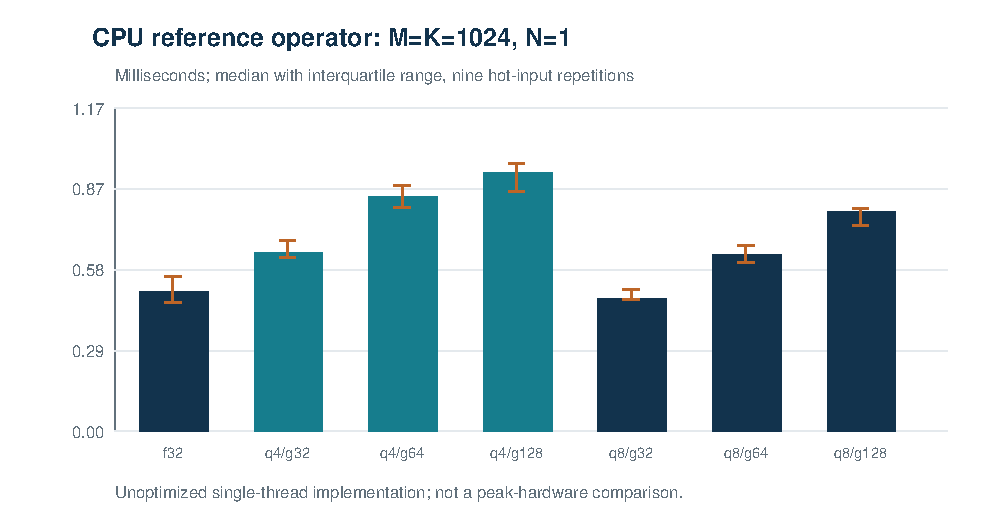
\includegraphics[width=0.95\linewidth]{figures/operator.pdf}
\caption{Actual CPU reference measurements. Error bars denote the IQR of nine
hot-input repetitions. The implementation is intentionally simple and is not an
optimized-library baseline.}
\label{fig:operator}
\end{figure}

\begin{table}[t]
\centering\small\begin{tabular}{lrrrr}
\toprule
Format & KiB & Median ms & IQR ms & Rel. MSE \\
\midrule
f32 & 4096 & 0.506 & 0.093 & 2.90e-13 \\
q4\_g32 & 640 & 0.647 & 0.064 & 1.80e-02 \\
q4\_g64 & 576 & 0.846 & 0.080 & 2.97e-02 \\
q4\_g128 & 544 & 0.932 & 0.104 & 4.27e-02 \\
q8\_g32 & 1152 & 0.480 & 0.037 & 5.29e-05 \\
q8\_g64 & 1088 & 0.639 & 0.061 & 7.98e-05 \\
q8\_g128 & 1056 & 0.795 & 0.062 & 1.19e-04 \\
\bottomrule
\end{tabular}

\caption{Measured example: $M=K=1024$, $N=1$. Payload includes scales and padding.
Relative MSE compares outputs against original F32 weights.}
\label{tab:operator}
\end{table}

\subsection{Compression does not establish acceleration}
Table~\ref{tab:operator} and Figure~\ref{fig:operator} show a concrete counterexample
to treating nominal precision as a speed guarantee. Q4/G32 stores 640 KiB versus
4096 KiB for F32, a 6.4-fold payload reduction. Its measured median latency in this
pilot is nevertheless higher than the F32 reference. Within Q4, changing group size
changes both reconstruction error and runtime. These differences cannot be
attributed solely to external-memory traffic: data may reside in cache, decoding
and accumulation interact, and compiler-generated instructions were not profiled.

The comparison does not show that optimized four-bit execution is intrinsically
slow. It shows that a compression result and a claim about a concrete execution
path are separate propositions. Similarly, subtracting a streaming-copy benchmark
from this operator would not isolate a pure decode cost because access patterns
and overlap would differ.

\subsection{The quality constraint rejects mixed bitwidths}
All three synthetic networks have exactly 27 feasible configurations at the chosen
quality and storage constraints. Every feasible configuration uses eight-bit
weights in all three layers; the 27 possibilities arise from group choices.
Consequently, no result in this pilot demonstrates a mixed-bitwidth advantage.
The hardware-aware rule and the quality-only rule both select Q8/G32 in each layer
for each seed. Timing differences between those labels are repeated measurements
of identical computations, not gains attributable to selection policy.

\begin{table}[t]
\centering\small\begin{tabular}{rlrrr}
\toprule
Seed & Selection & Dev. MSE & Test MSE & CPU ms \\
\midrule
11 & Q4/G128 & 0.14275 & 0.14804 & 0.156 \\
11 & Q8/G64 & 0.00031 & 0.00033 & 0.133 \\
11 & HW-aware & 0.00019 & 0.00022 & 0.125 \\
23 & Q4/G128 & 0.14716 & 0.15306 & 0.152 \\
23 & Q8/G64 & 0.00032 & 0.00033 & 0.135 \\
23 & HW-aware & 0.00022 & 0.00022 & 0.130 \\
37 & Q4/G128 & 0.15434 & 0.15551 & 0.151 \\
37 & Q8/G64 & 0.00035 & 0.00033 & 0.144 \\
37 & HW-aware & 0.00023 & 0.00022 & 0.125 \\
\bottomrule
\end{tabular}

\caption{Development/test relative MSE and independently measured composed CPU
latency. HW-aware selects Q8/G32 in every layer for all three seeds. The Q4 baseline
violates the quality constraint and must not be treated as an eligible winner.}
\label{tab:search}
\end{table}

\begin{figure}[t]
\centering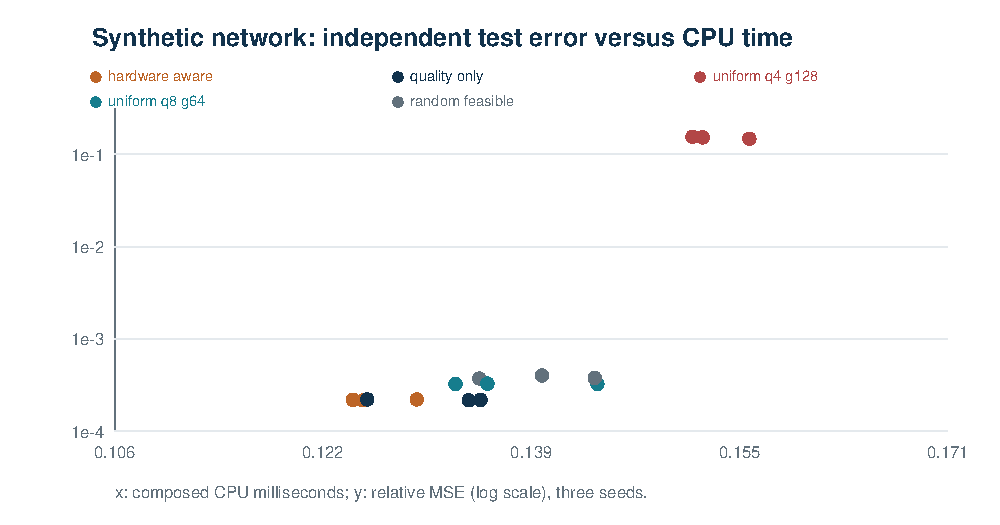
\includegraphics[width=0.95\linewidth]{figures/search.pdf}
\caption{Synthetic-network held-out error and composed timing. Three seeds and
separately measured repeated configurations expose uncertainty rather than
establishing a robust ranking between close timings.}
\label{fig:search}
\end{figure}

The additive cost proxy is not assumed to predict composed latency exactly. In
particular, native composition creates runner objects, copies intermediate outputs,
and applies tanh; these costs are absent from the per-layer lookup. The report
retains both predicted and actual times so that disagreements remain visible.
No calibration-error target or speedup claim is inferred from this small sample.
A larger, optimized experiment would need held-out timing validation and an
appropriate uncertainty model before using this cost function for architecture
recommendations.

\subsection{Hypothetical feature evaluation}
Figure~\ref{fig:architecture} illustrates how doubled decode throughput can lose
value when memory transfer, computation, or launch dominates. This behavior follows
from Equation~\ref{eq:time} and the disclosed parameters; it is not additional
hardware evidence. A feature with $S=1$ has no positive extra-area budget under
Equation~\ref{eq:area}. A feature with higher scenario speedup creates a conditional
budget, but the budget becomes actionable only after model calibration and area
estimation. No general recommendation to build a decoder follows from this pilot.

\begin{figure}[t]
\centering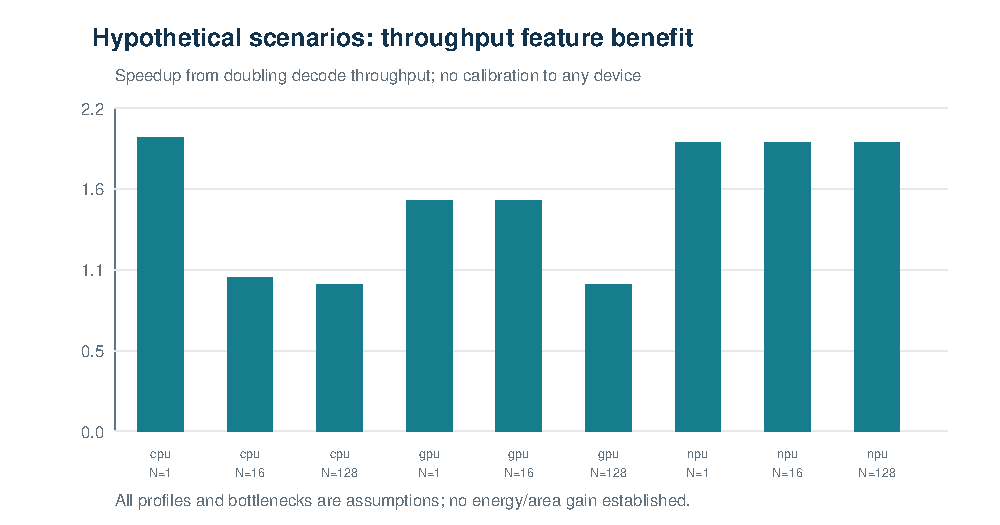
\includegraphics[width=0.95\linewidth]{figures/architecture.pdf}
\caption{Hypothetical feature sensitivity for Q4/G32, $M=K=1024$. Unlike the other
two figures, these points are uncalibrated scenarios, not measured execution.}
\label{fig:architecture}
\end{figure}

\section{Stage 2: Pretrained-Model Evidence on M4 Pro}
\subsection{Protocol and provenance}
We pin llama.cpp source commit \texttt{451b89bae0c4} and Qwen's official
Qwen2.5-1.5B-Instruct-GGUF repository revision \texttt{91cad51170dc}.
The full revisions and SHA-256 hashes for the
source archive, three model files and two datasets appear in the machine-readable
configuration and manifest. Model weights and datasets are not redistributed.

We build a CPU-only executable and a Metal-enabled executable with BLAS disabled.
CPU tests use eight threads and zero GPU layers. Metal tests request all model
layers on the accelerator. For each of F16, Q8\_0 and Q4\_K\_M, we run prompt
processing at prompt length $P\in\{128,2048\}$ and generation length $G=128$.
The token-block size used by llama.cpp is varied in the extended sweep but not
interpreted as request-level concurrency. Each cell contains seven llama-bench
repetitions; the execution order is deterministically shuffled. The benchmark
stores every sample and exact command. We do not flush caches, lock frequency, or
claim independent-session confidence intervals.

Quality evaluation uses the same three official model variants. We measure
perplexity on 32 context-512 chunks from the WikiText-2 raw test file and normalized
accuracy on 200 HellaSwag validation tasks with seed 1234. These sample sizes make
this a gate experiment rather than a definitive model-quality evaluation.

\subsection{The crossover moves with model scale and batching strategy}
We extended Stage 2 with a 72-case benchmark sweep across model size, backend,
prompt length, and token-block configuration. The matrix covers both Qwen2.5-1.5B
and Qwen2.5-7B GGUFs, CPU and Metal, prompt lengths of 128/512/2048 for 1.5B and
128/512/1024 for 7B, and token-block sizes of 1, 2, 4, 8, and 16 for prefill.
Decode cases use generation length $G=128$ and the same token-block sweep. The
measured trend is consistent with a moving crossover rather than a fixed universal
rule.

For the 7B model on CPU, 1024-token prefill rises from 6.35 token/s at the
smallest token block to 56.20 token/s at the largest measured block, whereas Metal
remains in the 36.8--46.9 token/s range for the same prompt length. The same trend
appears in shorter prompts: 128-token prefill runs at 28.75 token/s at the
smallest block versus 78.01 token/s at the largest block on CPU, whereas Metal
stays near 47.7--49.9 token/s. These data indicate that software block size can
materially alter the relative backend ranking, particularly in the prefill regime;
they do not isolate request-level concurrency as the underlying cause. The
inference policy therefore remains phase-aware rather than hardware-determined.

\subsection{Performance is phase dependent}
Table~\ref{tab:stage2-performance} and Figure~\ref{fig:stage2-performance} expose
the central result. On CPU, F16 is fastest for 2048-token prefill at 516.1 token/s,
while Q4\_K\_M is fastest for 128-token generation at 114.0 token/s, 2.78$\times$
F16. Q8\_0 sits between them at 419.7 token/s in prefill and 70.8 token/s in
decode. On Metal, F16 is again fastest for prefill at 1872.2 token/s, with Q8\_0
and Q4\_K\_M at 1530.4 and 1287.2 token/s respectively. The generation ranking
reverses: Q4\_K\_M reaches 121.3 token/s, 1.93$\times$ F16.

\begin{table}[t]
\centering\small\begin{tabular}{llrrr}
\toprule
Backend & Phase & F16 & Q8\_0 & Q4\_K\_M \\
\midrule
CPU & Prefill & 516.1 & 419.7 & 357.3 \\
CPU & Decode & 41.0 & 70.8 & 114.0 \\
METAL & Prefill & 1872.2 & 1530.4 & 1287.2 \\
METAL & Decode & 62.8 & 98.8 & 121.3 \\
\bottomrule
\end{tabular}

\caption{Measured Qwen2.5-1.5B throughput in token/s. Prefill uses 2048 tokens;
decode uses 128 generated tokens. Values are llama-bench means over seven samples.}
\label{tab:stage2-performance}
\end{table}

\begin{figure}[t]
\centering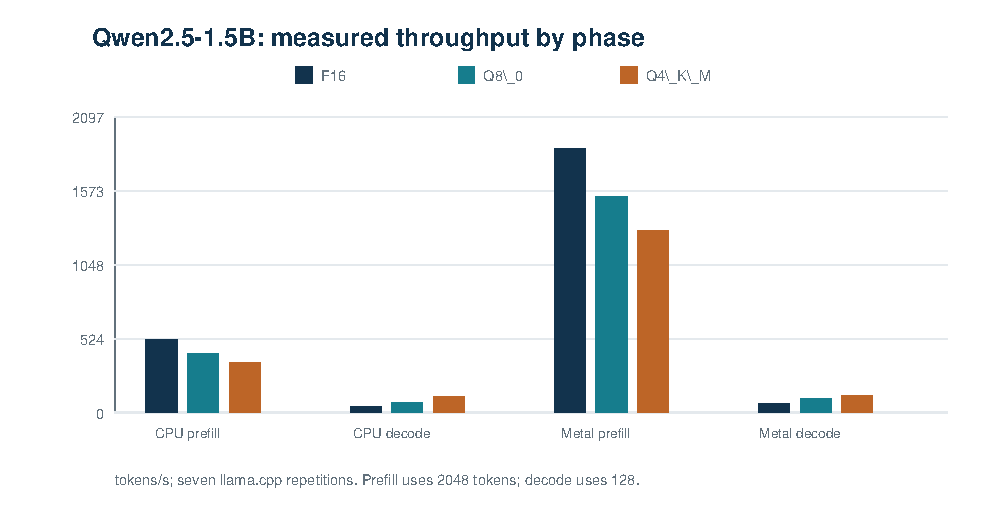
\includegraphics[width=0.97\linewidth]{figures/stage2-performance.pdf}
\caption{The fastest precision changes with execution phase and backend. Apple
Metal measurements are not Arm GPU measurements.}
\label{fig:stage2-performance}
\end{figure}

The phase reversal is evidence against specifying one preferred precision for the
whole inference lifecycle. It is consistent with decode benefiting from a smaller
streamed weight payload, while prefill can reward the throughput of a dense compute
path. Establishing the mechanism requires instruction and memory-counter profiles;
the timing matrix alone cannot attribute causality.

These measurements motivate a phase-aware software policy rather than a universal
hardware recommendation. In the present configuration, the relative ranking changes
with prompt length, token-block size, and backend, which suggests that a distinct
decode-optimized implementation may be valuable for some workloads. However, the
current evidence does not yet establish the required change in hardware substrate,
the end-to-end cost of format switching, or the benefit of dedicated on-chip
resources. The present project therefore supports a phase-aware design question;
it does not identify a final Arm GPU/NPU or heterogeneous microarchitecture.

\subsection{Quality gate and architecture verdict}
\begin{table}[t]
\centering\small\begin{tabular}{lrrr}
\toprule
Format & Size (GiB) & WikiText PPL & HellaSwag (\%) \\
\midrule
F16 & 3.32 & 8.9573 & 61.5 \\
Q8\_0 & 1.76 & 8.9524 & 61.5 \\
Q4\_K\_M & 1.04 & 9.3102 & 60.0 \\
\bottomrule
\end{tabular}

\caption{Official GGUF file size and measured quality pilots. HellaSwag uses 200
fixed-seed tasks; its 95\% intervals overlap across all three formats.}
\label{tab:stage2-quality}
\end{table}

Q8\_0 is effectively unchanged from F16 on both pilots. Q4\_K\_M reduces file size
from 3.32 to 1.04 GiB but raises perplexity from 8.9573 to 9.3102 (3.94\%) and
reduces HellaSwag accuracy from 61.5\% to 60.0\%. Because the HellaSwag intervals
overlap, the subset does not establish a statistically resolved accuracy difference.

The resulting design recommendation is conditional. The present evidence supports
phase-aware software selection: dense prefill should be preserved where compute is
limited, while compressed-weight decode may be favorable in the latency-sensitive
regime that dominates single-stream generation. A future Arm study should test
whether CPU SME/SVE2 kernels, an Arm GPU, and an NPU reproduce this boundary, and
should price any format conversion or decompression support in power and area. The
present evidence can reject a universal policy; it cannot yet select a specific
future Arm microarchitecture.

\section{Threats to Validity and Required Next Evidence}
\paragraph{Synthetic quality.}
The generated-network selection remains only a machinery test. Stage 2 adds one
pretrained 1.5B model family, but its 32 perplexity chunks and 200 HellaSwag tasks
do not cover instruction following, long context, other architectures, or broad
statistical variation. Full test sets and a second model family are required.

\paragraph{Software baseline.}
The scalar code is a reference, not a demonstration of optimized Arm execution.
Memory scheduling, vectorized unpacking, matrix instructions, scale fusion, and
library-specific packing may change all observed rankings. No SME/NEON claim is
made without instruction-path evidence. FP32 activations also differ from many
integer accelerator interfaces; converting them introduces additional numerical
and execution questions.

\paragraph{Measurement.}
We measured a single session with hot data, nine within-block repetitions, and no
frequency or thermal controls. Timing includes Python dispatch. Small differences
may reflect drift and fixed overhead. The appropriate next step is randomized,
multi-session measurement with a clearly stated cache regime, thread policy,
clock/thermal observations, and optimized comparison paths. We do not interpret
these results as request-concurrency effects unless independent requests are
measured explicitly.

\paragraph{Cross-platform coverage.}
Metal now executes both the custom reference and llama.cpp workload on this host.
Apple GPU evidence is still not evidence for an Arm GPU. The NPU checker is only an
illustrative static contract inspection; real compilation, partition logs, fallback
behavior, and target execution or validated simulation are required.

\paragraph{Architecture, energy, and area.}
The scenario profiles are not product specifications. There is no calibrated PPA
model and no memory-hierarchy traffic measurement. No power domain was measured,
and no RTL was synthesized. A dedicated decoder should be evaluated against an
optimized software alternative, then costed with explicit throughput, buffering,
flow-control, clock and synthesis constraints. The normalized area bound should
only be compared with a correspondingly scoped area measurement.

\section{Conclusion}
EdgeDecode connects a transparent operator study to real pretrained-model evidence.
Across the measured workloads, the preferred precision is not fixed: Q4\_K\_M
wins single-stream decode, whereas F16 remains best for long-context prefill on the
hosted Metal path. The crossover shifts again as model scale, token-batching
strategy, and prompt length vary, indicating that the correct interpretation is
phase-aware rather than globally low-precision. The quality gate shows that Q8\_0
remains close to F16, while Q4\_K\_M trades model fidelity for memory efficiency
in a way that is favorable largely in the decode regime. The immediate design
implication is therefore not a universal datapath but a workload-dependent policy:
the best-performing implementation depends on the active bottleneck. Arm
validation, hardware counters, power measurement, and synthesized area remain
necessary before translating this rule into a product proposal.

\section*{Artifact Availability and Disclosure}
The accompanying source repository contains native kernels, Python code, tests,
raw timing samples, every search candidate, source hashes, hypothetical parameter
files, and figure/table generators. Commands are documented in the repository
README. No pretrained weights or external datasets are redistributed. Code and
original documentation use the MIT license. The draft and implementation were
prepared with AI assistance and require human review before external submission.
No institutional affiliation or hardware-vendor endorsement is implied.

\begin{thebibliography}{9}
\bibitem{haq} K. Wang, Z. Liu, Y. Lin, J. Lin, and S. Han.
HAQ: Hardware-Aware Automated Quantization with Mixed Precision.
CVPR, 2019. \url{https://arxiv.org/abs/1811.08886}.
\bibitem{awq} J. Lin et al.
AWQ: Activation-aware Weight Quantization for On-Device LLM Compression and Acceleration.
MLSys, 2024. Original paper version:
\url{https://arxiv.org/abs/2306.00978v4}.
\bibitem{roofline} S. Williams, A. Waterman, and D. Patterson.
Roofline: An Insightful Visual Performance Model for Multicore Architectures.
Communications of the ACM, 52(4):65--76, 2009.
\url{https://doi.org/10.1145/1498765.1498785}.
\bibitem{kleidiai} Arm contributors. KleidiAI: optimized compute routines for Arm CPUs.
Source repository, accessed September 10, 2026.
\url{https://github.com/ARM-software/kleidiai}.
\end{thebibliography}
\end{document}
